\chapter{評価実験}
\thispagestyle{fancy}


\section{評価方法}
図\ref{kankyou}のようにプロジェクターとKinectを配置する.
体験者はKinectの正面に立つ.

本研究で提案したプロジェクションマッピングの評価を得るために,
5名の被験者に体験してもらい,アンケートを実施した.

\vspace{1cm}
\begin{figure}[h]
  \centering
  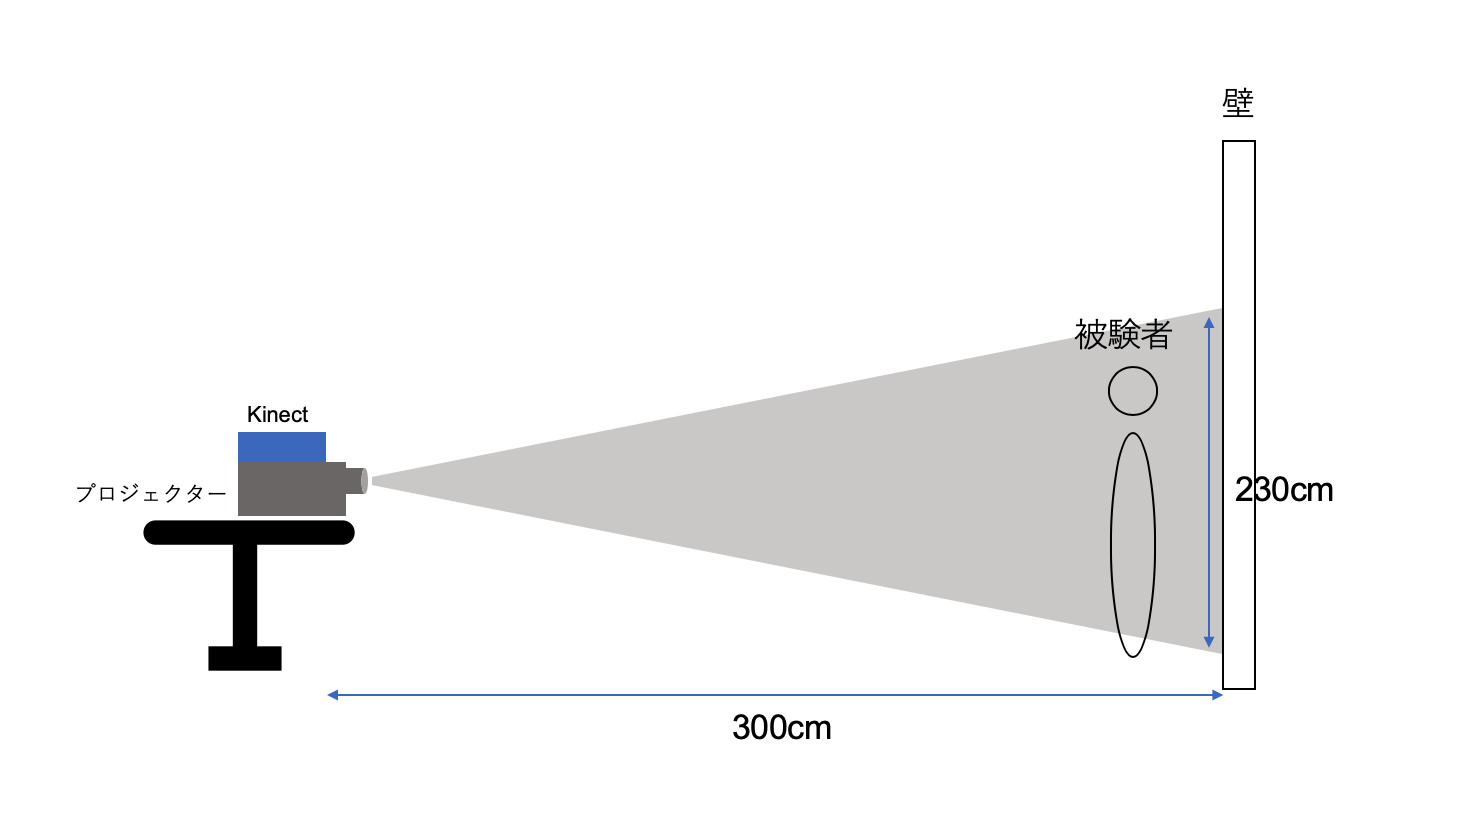
\includegraphics[width=14cm]{image/jikkenkankyou.png}
  \caption[評価実験環境図]{評価実験環境図.}
\label{kankyou}
\end{figure}


\clearpage

アンケートの質問内容を以下に示す.
\begin{itemize}
  \item[Q1.] 操作はわかりやすいか? [5段階評価]
  \item[Q2.] わかりづらかった場合,どこがわかりづらいか? 
  \item[Q3.] 楽しさについての満足感はどれくらいか? [5段階評価]
  \item[Q4.] 今後の改善点や意見・要望   
\end{itemize}



\section{評価結果}
図\ref{hyouka}にアンケート結果を示す.

Q1の操作のわかりやすさに関しては平均4点を得ることができた.

Q2のわかりにくかった部分では「操作方法が口頭での説明だったので,教えてもらうまでわからなかった.」
という回答が得られた.

Q3の楽しさに対する満足度に関しては平均4.2点を得ることができた.

Q4の今後の改善点や意見・要望に関しては以下の回答が得られた.
\begin{itemize}
  \item 「ボールをリアルにして欲しい」
  \item 「膝以外でもリフティングしたい」
  \item 「観客の声援が欲しい」
  \item 「回数表示機能が欲しい」
  \item 「チュートリアルが欲しい」
  \item 「音に臨場感が欲しい」
  \item 「何かゲーム性が会ったらもっと楽しめると思う」
  \item 「認識が上手くいかなかった」
  \item 「ボールが遅くなっている点が気になった」
  \item 「卓球verも追加して欲しい」
  \item 「もうちょっとFPSを上げて欲しい」
\end{itemize}


\begin{figure}[p]
  \centering
  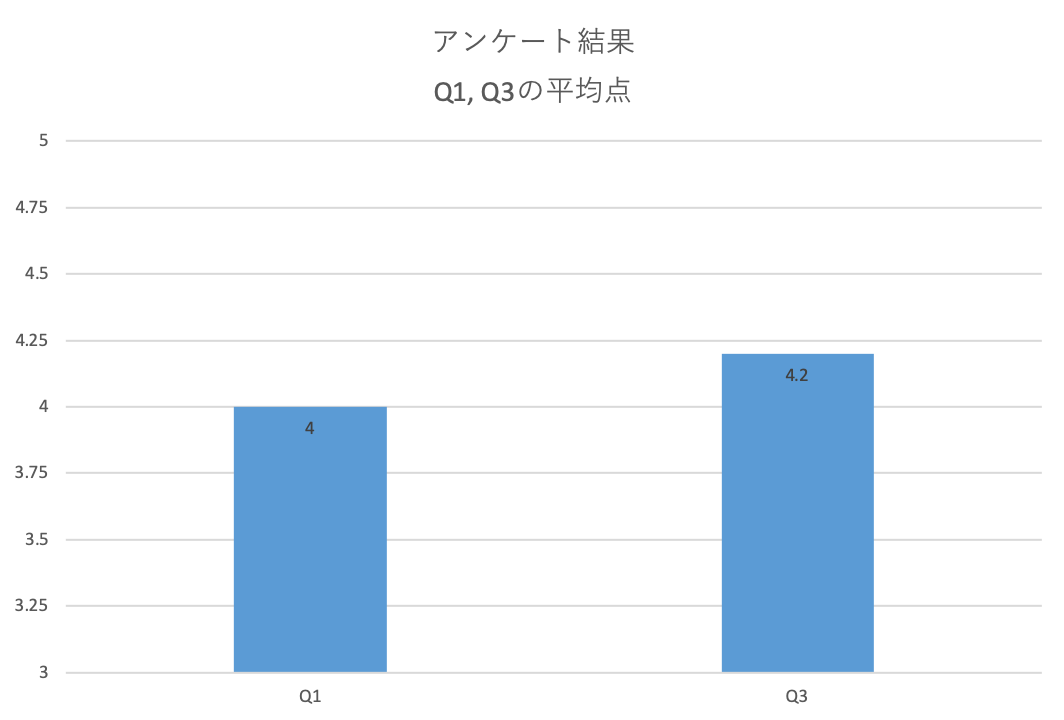
\includegraphics[width=12cm]{image/ave.png}
  \caption[アンケート結果]{アンケート結果.}
\label{hyouka}
\end{figure}
